%
% Copyright (c) 2023 Aleksey Fedoseev <aleksey@fedoseev.net>
% 
% Permission is granted to copy, distribute and/or modify this document
% under the terms of the GNU Free Documentation License, Version 1.3
% or any later version published by the Free Software Foundation;
% with no Invariant Sections, no Front-Cover Texts, and no Back-Cover Texts.
% A copy of the license is located here: http://www.gnu.org/copyleft/fdl.html.
%

\documentclass[12pt,a4paper]{article}
\usepackage[T2A]{fontenc}
\usepackage{ucs}
\usepackage[utf8]{inputenc}
\usepackage[english,russian]{babel}
\usepackage{indentfirst}
\usepackage{amsmath}
\usepackage{amssymb}
\usepackage{gensymb}
\usepackage{graphicx}
\usepackage{hyperref}
\usepackage{array}
\usepackage{titlesec}
\usepackage{subcaption}
\usepackage{wasysym}
\usepackage{longtable}
\usepackage{multirow}

\pagestyle{plain}
\parindent=1.25cm
\textheight=24cm
\textwidth=16cm
\topmargin=-1cm
\frenchspacing
\renewcommand{\theequation}{\thesection.\arabic{equation}}
\newcommand{\sectionbreak}{\clearpage}

\begin{document}

\title{%
  \textbf{Иерархические машины состояний для программ полета космических аппаратов} \\
    Руководство по программированию для инженерного симулятора ОРБИТА 2.0}

\author{
  Алексей Федосеев\\
  \texttt{aleksey@fedoseev.net}
}

\date{Версия 1.0, \today}

\maketitle

Этот текст распространяется под лицензией GNU Free Documentation License (FDL) версии
1.3. Подробную информацию об этой лицензии Вы можете на сайте GNU
\footnote{\url{http://www.gnu.org/copyleft/fdl.html}}.

Исходный текст находится в репозитории проекта на GitHub
\footnote{\url{https://github.com/dralex/orbita-simulator}}.

\tableofcontents

\clearpage
\section{Введение}

Это руководство дополняет \textbf{Руководство для преподавателя для инженерного симулятора
  ОРБИТА 2.0} и знакомит с графическим языком \emph{иерархических машин состояний} в
применению к созданию программ полета для спутников на орбите Земли в рамках
симулятора. Для общего знакомства с диаграммами машин состояний лучше обратиться к
специализированным книгам и статьям (например, \cite{CRASHCOURSE}) или описанию диаграм
Statecharts в стандарте UML 2.0.

Руководство состоит из разбора примеров диаграмм программ полета для миссий, входящих в
базовую версию симулятора ОРБИТА 2.0: начиная с трёх тренировочных миссий и заканчивая
самыми сложными финальными миссиями. Исходные файлы диаграмм и описаний аппаратов можно
найти в директории \verb'probes' репозитория.

В симуляторе используются программы полета на языке Python (версия 3.x) с использованием
специального API для доступа к подсистемам аппарата, подробнее об этом сказано в разделе
\textbf{Создание программ полета на языке Python} основного руководства к ОРБИТЕ 2.0. Для
того, чтобы использовать диаграммы машин состояний в качестве программ полета необходимо:

\begin{description}
\item[Редактор диаграмм] Редактор необходим для редактирования и сохранения диаграмм в
  виде \verb'.graphml'-файла. На данный момент поддерживаются только диаграммы, созданные
  в бесплатном, но проприетарном редакторе
  \textbf{yEd}\footnote{\url{https://www.yworks.com/products/yed}}.
\item[Транслятор диаграмм в программу полета на Python] В данной версии симулятора
  используется транслятор в код Python с применением библиотеки машин состояний
  \textbf{PySM}\footnote{\url{https://github.com/pgularski/pysm/}}. В журнале полета можно
  увидеть код программы, который генерируется на основе предложенной диаграммы.
\end{description}

Таким образом, вы можете создать диаграмму в \textbf{yEd}, следуя установленным правилам
оформления, а затем автоматически сгенерировать код программы на Python при запуске
симулятора, то есть вести всю разработку программы полета в графическом редакторе. Этот
путь содержит свои ограничения: придется внимательно следить за правильностью кода на
Python, зато разработчику вообще не потребуется работать с генерируемым исходным кодом
программы.

\clearpage
\section{Смотрим на Землю: знакомство с машинами состояний}

\paragraph{Условия миссии} В первой тренировочной миссии КА стартует на орбите заданной высоты. Необходимо погасить
начальное вращение аппарата и совершить полный оборот Земли с ориентацией аппарата в надир
(нормально по отношению к поверхности). В этой тренировочной миссии аппарат будет
полностью сконструирован, нужно будет только произвести расчёты и вставить в программу
полёта нужные константы.

\begin{figure}[tbh]
  \begin{center}
    \includegraphics[width=10cm]{images/test1-ru.eps}
    \caption{Положения аппарата в первой тренировочной миссии}
    \label{Pic:test1}
  \end{center}
\end{figure}

\paragraph{Общая логика решения} Напомним, что программу полета в данной миссии можно разделить на два этапа:

\begin{enumerate}
\item Гашение начальной угловой скорости аппарата и выход на угловую скорость, необходимую
  для постоянного поддержания нормальной к земной поверхности ориентации, целевую угловую
  скорость, необходимое время и момент маховика для совершения маневра вычисляются по
  формуле:

  $$
  \begin{array}{l}
    \omega = \frac{-360 \degree \sqrt{\frac{G M}{R + h_{\text{орб}}}}}{2 \pi (R + h_{\text{орб}})},\\
    t = \frac{2 \cdot 270 \degree}{\omega_0 - \omega},\\
    M_0 = \frac{(\omega - \omega_0) \cdot I_z}{t}.
  \end{array}
  $$
\item Поддержание аппарата в нужной ориентации и угловой скорости.
\end{enumerate}

\paragraph{Диаграмма состояний}

\begin{figure}[tbh]
  \begin{center}
    \includegraphics[width=16cm]{images/test1-sm.eps}
    \caption{Диаграмма машины состояний для миссии <<Смотрим на Землю>>}
    \label{Pic:Test1SM}
  \end{center}
\end{figure}

Такая последовательность этапов работы позволяет построить простую диаграмму машины
состояний нашего КА (см. \verb'test1sm.graphml'). Взглянем на диаграмму (рисунок
\ref{Pic:Test1SM}) и выделим ее ключевые составляющие.

На диаграмме представленна иерархия состояний:

\begin{description}
\item[orientation] Родительское состояние, характеризующее весь процесс ориентации
  аппарата.
\item[rotate] Первое дочернее состояние, связанное с начальным маневром.
\item[maintain] Второе дочернее состояние, связанное с последующим поддержанием правильной
  ориентации аппарата.
\item[idle] На очередном уровне иерархии базовое состояние связано с ожиданием, когда
  ориентация аппарата не требует корректировки.
\item[correct] И второе состояние, связанное с корректировкой угловой
  скорости\footnote{Обращаем внимание, что здесь реализован не самый лучший способ
    регулирования параметра. Лучше использовать более сложный регулятор для пересечения
    границы значения, чтобы избежать <<дребезга>> при переходе. Например, вы можете подумать
    над диаграммой для более сложного переходного процесса, ПИД-регулятора и т.п.}, в том числе:
\item[correct\textunderscore cw] Дочернее состояние, корректирующее превышение угловой
  скорости по часовой стрелке.
\item[correct\textunderscore ccw] И аналогично~--- против часовой стрелки. 
\end{description}

Также на диаграмме можно увидеть начальное состояние для всей диаграммы (мы начинаем
выполнение с того, что попадаем в состояние \verb'rotate') и отдельно для ситуации
попадание в состояние \verb'correct'.

Состояние содержат триггеры (\emph{trigger}) на вход (\verb'entry') и выход (\verb'exit'), в которых
указывает исполняемый код на Python. В коде происходит обращение к подсистемам КА,
описанным в справочнике по программированию в основном руководстве к ОРБИТЕ 2.0. Например,
при входе в состояние  \verb'correct' маховик включается

\begin{verbatim}
orientation.start_motor(AXIS_Z)
\end{verbatim}

а при выходе~--- выключается:

\begin{verbatim}
orientation.stop_motor(AXIS_Z)
\end{verbatim}

Переход между состояниями происходит посредством событий (переход, \emph{transition}). В
данном примере используются только так называемые \emph{внешние события}, связанные с
изменением текущего состояния. Каждое событие содержит:

\begin{description}
\item[Название] Названия события пишется латинскими буквами. Мы будем (и рекомендуем)
  использовать нотацию, в которой названия событий пишутся заглавными буквами. Может не
  указываться, в этом случае считается, что это стандартное событие \verb'TIME_TICK'. Мы
  не рекомендуем злоупотреблять событиями без названий.
\item[Условие] В случае истинности условия (\emph{guard}) происходит переход. Условия
  также представляет сбой код на языке Python, заключенный в квадратные скобки. Если
  переход не содержит условия, он происходит безусловно. Пример такого кода в диаграмме:
  \verb'[abs(orientation.get_angular_velocity(AXIS_Z) - W) < DW]'.
\item[Действие] Возможно также выполненение специального действия (\emph{action}) в
  процессе перехода (если условие истинно)~--- до того, как система перейдет в новое
  состояние. Действие представляет собой код программы на языке Python в виде строк после
  символа \verb'/'. Например: \verb'/ orientation.stop_motor(AXIS_Z)'.
\end{description}

Также диаграмма содержит специальные заметки~--- блоки желтого цвета со служебными
заголовками.

\begin{description}
\item[Initialization:] Блок инициализации, сюда помещается код программы полета,
  который будет выполнен до входа в диаграмму. В случае программы на Python здесь удобно
  проводить стартовые вычисления и располагать инициализацию глобальных переменных,
  которые затем будут использоваться в программе. Например\footnote{Обратите внимание, что в нашем
    примере указаны какие-то значения для переменных $t$, $M0$ и др., скорее всего они не
    приведут к корректному выполнению программы миссии, для этого вам нужно самостоятельно
    провести корректные расчеты.}:

\begin{verbatim}
Initialization:

T = 508
W = -0.06
M0 = -0.00001
M = 0.000001
DW = 0.00001
\end{verbatim}

\item[Init scripts:] Альтернативный способ добавления кода в диаграмму~--- перечисление
  файлов с кодом на питоне, которые будут импортированы со всеми символами в генерируемую программу
  полета. \textbf{Обратите внимание:} все скрипты должны находиться в той же директории,
  что и \verb'.graphml'-файл. Пример содержания блока:

\begin{verbatim}
Init scripts:

constants.py
orientation.py
\end{verbatim}

\end{description}

При генерации кода программы полета сперва включаются все модули из блока
\verb'Init scripts', а затем код из блока \verb'Initialization'. Это позволяет более
логично распределять код между блоками и диаграммами нескольких подсистем (см. пример на
странице \pageref{MULTIPLE_MODULES}).
 
\paragraph{Особенности написания кода в диаграммах} Данный подход имеет ряд особенностей
написания кода, которые нужно учитывать при создании программы полета.

Во-первых, парадигма программирования машин состояний наиболее эффективна, если основное
время программы ничего не происходят, а управляющие воздействия осуществляются в момент
возникновения событий и занимают относительно мало времени. Это значит, вам нужно
постараться минимизировать объем кода (вычислений, обращений к внешним устройствам и пр.)
при выполнении отдельных событий, проверке условий, срабатывании триггеров и
т.п. Например, части сложных вычислений можно произвести заранее и вынести их в блок
инициализации.

Во-вторых, редактор \textbf{yEd} не предназначен для написания большого объема текста. В нем нет
встроенных механизмов проверки синтаксиса на Python и других удобных инструментов для
разработчика. А значит, вам нужно внимательнее писать код и отлаживать диаграмму уже  при
запуске аппаратов. Не забывайте про тестовую библиотеку \textbf{Sputnik API}, которую
можно совместить с отладкой диаграмм состояний
(см. \verb'/models/earth/sm/test'). Подробнее про систему тестирования диаграмм можно
прочитать в Приложении 1.

\clearpage
\section{Связь с Землей: использования событий}

\paragraph{Условия миссии} Во второй тренировочной миссии КА стартует на орбите заданной высоты. Необходимо
запрограммировать аппарат для отправки сообщения на Землю через подсистему
высокопроизводительной связи. В этой тренировочной миссии аппарат будет полностью
сконструирован, нужно будет только написать его программу полёта.

\begin{figure}[tbh]
  \begin{center}
    \includegraphics[width=10cm]{images/test2.eps}
    \caption{Аппарат и НИП во второй тренировочной миссии}
    \label{Pic:test2}
  \end{center}
\end{figure}

Эта миссия принципиально не отличается от предыдущей. Необходимо не только сориентировать
аппарат на Землю, но и передать сообщение на Землю в момент, когда аппарат приблизится к
точке расположения НИП на Земле.

\paragraph{Общая логика решения} С точки зрения программирования полета с помощью машин
состояний в этой миссии мы плотнее поработаем с \emph{событиями} и покажем, как можно
управлять миссией КА при помощью нескольких диаграмм состояний.

В данном случае миссию можно разделить на три этапа:

\begin{enumerate}
\item Сориентировать аппарат в надир, чтобы антенна с углом направленности
  $180\degree$ была сориентирована максимально в сторону цели.
\item Дождаться момента, пока НИП покажется из-за горизонта.
\item Включить передатчик и передать нужное сообщение.
\end{enumerate}

Одновременно с этим в миссии необходимо поддерживать температурный режим аппарата, что
потребует отдельной диаграммы для соответствующей подсистемы КА.

\paragraph{Ориентация аппарата}

\begin{figure}[tbh]
  \begin{center}
    \includegraphics[width=16cm]{images/test2sm-orient-1.eps}
    \caption{Диаграмма машины состояний для подсистемы ориентации (а)}
    \label{Pic:Test2SM-Orient-1}
  \end{center}
\end{figure}

Сперва познакомимся с диаграммой, которая обеспечивает ориентацию КА. Она в целом
наследует диаграмму из прошлой миссии~--- на рисунке \ref{Pic:Test2SM-Orient-1}) показана
первая часть нашей диаграммы. В ней есть пара отличий: во-первых, константы для первого
поворота теперь вычисляются в зависимости от текущего движения аппарата; во-вторых, часть
условий были спрятаны в функции на языке Python; но самое главное~--- здесь появляется
новая логика, связанная с передачей сообщения между различными диаграммами подсистем КА.

При получении внешнего сообщения \verb'TO_NADIR' система ориентации начинает стартовый
поворот в надир. А по окончанию маневра в другую подсистему (в данном случае \verb'cpu')
отправляется соответствующее сообщение:

\begin{center}
\begin{verbatim}
DISPATCH(cpu, 'ORIENTED')
\end{verbatim}
\end{center}

\verb'DISPATCH'~--- это служебная функция, которая отправляет сообщение в эту или другую
подсистему КА. Функция принимает два параметра:

\begin{description}
\item[Название подсистемы] в которую отправляется сообщение, в данном случае это БЦВМ
  (\verb'cpu').
\item[Название сообщения] которое должно обрабатываться в диаграмме соответствующей
  подсистемы в виде строки, в данном случае \verb"'ORIENTED'".
\end{description}

Далее представлен код инициализации, который используется в машине состояний для
подсистемы ориентации. В служебных полях содержится код инициализации, включая необходимые
функции для вычислений и проверки условий.

\begin{verbatim}
Initialization:

mass = 5.5
volume = 3.4
a = math.pow(volume, 1.0 / 3.0) / 10.0
I_z = (1.0/12.0) * (2.0 * a ** 2) * mass
GM = 6.6742e-11 * 5.9726e24 
R_z = 6371032.0

def calculate_nadir_rotation():
    h = navigation.get_orbit_height()
    w0 = orientation.get_angular_velocity(AXIS_Z)

    w = -360.0 * math.sqrt(GM / (R_z + h)) / (2 * math.pi * (R_z + h))
    t = 2 * 270.0 / (w0 - w)
    m0 = (w - w0) * I_z / t

    return w, t, m0

def is_target_dw():
    return abs(orientation.get_angular_velocity(AXIS_Z) - W) < DW

def is_target_oa():
    a = navigation.get_z_axis_angle()
    oa = orientation.get_angle(AXIS_Z)
    sum = a + oa
    if sum >= 360.0: sum = sum - 360.0
    return abs(sum - 270.0) < DA

M = 0.000001
DW = 0.00001
DA = 0.01
Start_T = 0
\end{verbatim}

\paragraph{Основная диаграмма} БЦВМ содержит собственно программу полета в виде следующей
диаграммы (см. рисунок \ref{Pic:Test2SM-Main}).

\begin{figure}[tbh]
  \begin{center}
    \includegraphics[width=15cm]{images/test2sm-main.eps}
    \caption{Диаграмма машины состояний для центрального процессора}
    \label{Pic:Test2SM-Main}
  \end{center}
\end{figure}

В этой диаграмме последовательно реализуются три этапа полета: сперва посредством отправки
сообщения с подсистему ориентации инициируется поворот в надир. Затем, после завершения
поворота, КА переходит в режим ожидания НИП-а, после чего переходит в состояние, связанное
с отправкой сообщения.

Итого, КА может содержать независимо работающие программы для отдельных подсистем. Внутри
подсистемы и между подсистемами можно пересылать события с помощью
\verb'DISPATCH'. \textbf{Обратите внимание}, что название верхнеуровневого состояния в
каждой из диаграмм совпадает с названием подсистемы. Это не случайно! Для корректной
отправки и получения событий между подсистемами вам необходимо использовать это требование
к именованию состояний в диаграммах для программ отдельных подсистем.

\paragraph{Температурный режим} Третья диаграмма связана с работой подсистемы обеспечения
теплового режима аппарата. Следующая диаграмма (рисунок \ref{Pic:Test2SM-Therm}) содержит
переход между состояниями ожидания и нагрева аппарата, если потребуется повысить его
температуру в следствие естественного охлаждения.

\begin{figure}[tbh]
  \begin{center}
    \includegraphics[width=15cm]{images/test2sm-therm.eps}
    \caption{Диаграмма машины состояний для поддержания необходимой температуры КА}
    \label{Pic:Test2SM-Therm}
  \end{center}
\end{figure}

В этой диаграмме представлено особое событие \verb'TIMER_1M'. Это служебное событие,
которое срабатывает не на каждом шаге симулятора, а регулярно во времени, в данном случае
один раз в минуту. В данном случае у нас нет необходимости отслеживать тонкие изменения
температуры на коротких интервалах времени, достаточно раз в минуту проверять температуру
и при необходимости менять состояние подсистемы.

Пришло время рассмотреть служебные события, которые можно использовать в диаграммах, это:

\begin{itemize}
\item \verb'TIME_TICK'~--- срабатывает на каждом шаге симулятора; этому событию соответствуют
  также все неименованные события;
\item \verb'TIMER_1S', \verb'TIMER_1M', \verb'TIMER_1H'~--- срабатывают по таймеру раз в
  секунду, раз в минуту и раз в час, соответственно.
\end{itemize}

\paragraph{Выводы} Таким образом, вы можете использовать различные события в диаграммах, а
также создавать программы полета из нескольких взаимодействующих или полностью независимых
диаграмм, привязанных к отдельным подсистемам аппарата. В симуляторе ОРБИТА 2.0 все эти
программы исполняются параллельно (как если бы каждая работала на отдельном контроллере) и
являются некоторым аналогом ортогональных диаграмм из UML 2.0. В последующих, более
сложных миссиях мы будем все чаще обращаться к такому подходу.

\clearpage
\section{Орбитальный маневр: продолжаем изучать события}

\paragraph{Условия миссии} В последней из тренировочных миссий КА стартует на орбите
заданной высоты. Необходимо запрограммировать аппарат для перехода на более высокую
орбиту. Аппарат снова будет полностью сконструирован, нужно будет только рассчитать
необходимую массу топлива и написать программу полёта.

\begin{figure}[tbh]
  \begin{center}
    \includegraphics[width=12cm]{images/maneuvre.eps}
    \caption{Изменение орбиты КА посредством двухимпульсного перехода}
    \label{Pic:Maneuvre}
  \end{center}
\end{figure}

\paragraph{Общая логика решения} Мы будем использовать орбитальный переход с двумя
импульсами, который подробно описан в основном руководстве к
симулятору. Последовательность действий при орбитальным переходе можно разделить на
следующие шаги:

\begin{enumerate}
\item сориентировать аппарат тангенциально и погасить стартовую угловую скорость;
\item задать первый импульс;
\item развернуть аппарат и дождаться момента, когда аппарат окажется на противоположной
  стороне Земли;
\item задать второй импульс;
\item подождать полного оборота уже на новой орбите.
\end{enumerate}

При решении этой задачи мы введем несколько новых приемов, которые завершат наше
знакомство с машинами состояний для симулятора ОРБИТА 2.0. Первый из них~--- развитие
пересылки событий внутри и между машинами состояний.

\paragraph{События с параметром}

События внутри машины состояний или между двумя машинами можно передавать вместе с
параметром. Для этого можно использовать функцию \verb'DISPATCH_VALUE'. Эта функция похоже
на уже рассмотренную ранее \verb'DISPATCH', только в качестве третьего параметра
необходимо передать значение. На диаграмме машины (рисунок \ref{Pic:Test3SM-Navi})
состояний для системы навигации можно увидеть передачу состояния с параметром.

\begin{figure}[tbh]
  \begin{center}
    \includegraphics[width=16cm]{images/test3sm-navi.eps}
    \caption{Диаграмма машины состояний для подсистемы навигации}
    \label{Pic:Test3SM-Navi}
  \end{center}
\end{figure}

\label{MULTIPLE_MODULES}
Код программы навигации содержится в двух файлах \verb'test3sm_constants.py' и
\verb'test3sm_navi.py'.

Здесь используется пересылка сообщения \verb'TANGENT' в подсистему ориентации со значением
$180$: 

\begin{verbatim}
DISPATCH_VALUE(orientation, 'TANGENT', 180)
\end{verbatim}

Идея в том, что подсистема ориентации должна развернуть КА тангенциально, и завершить
данный переход в точке, в которой будет совершаться импульс двигателем, в данном
случае~--- в положении $180 \degree$ относительно оси $Z$.

В этой же диаграмме можно увидеть, как обрабатываются события с параметром. При получении
события \verb'TRANS_ORBIT(h)' используется значение высоты орбиты, на которую необходимо
перевести аппарат, высота задается в переменной $h$. \textbf{Обратите внимание},
переменная события может использоваться только в условии (\emph{guard}) или действии
(\emph{action}), связанных с данным переходом. Поэтому вам нужно ее как-то сохранить или
немедленно использовать. При передаче событий значения сохраняются в виде строк, поэтому
вам нужно будет осуществить обратную конвертацию в коде обработчика.

В следующей диаграмме подсистемы ориентации (рисунок \ref{Pic:Test3SM-Orient}) также показана
обработка событий со значением.

\begin{figure}[tbh]
  \begin{center}
    \includegraphics[width=16cm]{images/test3sm-orient.eps}
    \caption{Диаграмма машины состояний для подсистемы ориентации}
    \label{Pic:Test3SM-Orient}
  \end{center}
\end{figure}

Код программы ориентации содержится в двух файлах \verb'test3sm_constants.py' и
\verb'test3sm_orient.py'. Обратите внимание, что хранение кода диаграмм в файлах позволяет
объединять общие константы и методы программы полета в одном месте.

Сам поворот осуществляется в три последовательных этапа (гашение вращения, первая половина
поворота с разгоном и вторая половина поворота с торможением), после чего подсистема
ориентации переходит в режим ожидания и поддерживает нулевую угловую скорость. Обратите
внимание, что после завершения ориентации соответствующее событие отправляется в две
подсистемы аппарата (хотя это и не является необходимым, как мы увидим далее).

\begin{figure}[tbh]
  \begin{center}
    \includegraphics[width=11cm]{images/test3sm-main.eps}
    \caption{Диаграмма машины состояний для БЦВМ}
    \label{Pic:Test3SM-Main}
  \end{center}
\end{figure}

В главной программе полета (рисунок \ref{Pic:Test3SM-Main}) также можно увидеть применение
события со значением~--- при старте орбитального перехода, за который отвечает подсистема
навигации, ведь она связана с движением центра масс аппарата.

По завершению программы подсистема ориентации приводится в состояние бездействия с помощью
команды \verb'STOP'.

\begin{figure}[tbh]
  \begin{center}
    \includegraphics[width=12cm]{images/test3sm-heat.eps}
    \caption{Диаграмма машины состояний для регуляции температуры КА}
    \label{Pic:Test3SM-Heat}
  \end{center}
\end{figure}

\paragraph{Внутренние события}

Последнияя из важных языковых конструкций диаграммы машин состояний~--- \emph{внутренние
  события}. До этого мы с вами работали с переходами, которые меняют текущее состояние машины
состояний. Иногда нет необходимости менять состояние, но необходимо отреагировать на
внешний или внутренний сигнал.

Диаграмма подсистемы обеспечения теплового режима КА (рисунок \ref{Pic:Test3SM-Heat})
содержит внутреннее событие в рамках состояния \verb'heat'. Внутренние события напоминают
действия \verb'entry' и \verb'exit', но могут содержать не только действия, но и
условия\footnote{Обратите внимание, в данной реализации генератора кода для Python для
  внутренних событий необходимо указывать символ \textbf{/} без предварительных
  пробелов.}. В данном случае событие будет вызываться ежеминутно для изменения мощности
обогревателя~--- так мы добьемся более гладкой кривой перехода.  

\paragraph{Выводы}

В данной миссии мы перешли на более универсальный подход к написанию программ полета: код
программ на Python хранится в фалах и не утяжеляет схему. Отдельные действия КА
логически разделяются по подсистемам, управление которыми происходит через события.

Теперь вы знаете все возможности иерархических машин состояний и можете взяться за
диаграммы программ полета к основным миссиям симулятора.

\section{Дистанционное зондирование Земли}

\paragraph{Условия миссии} В этой миссии КА стартует на орбите
заданной высоты и будет полностью сконструирован. Необходимо сделать снимок объекта, расположенного на Земле, из космоса. Данные снимка нужно передать в наземный измерительный пункт (\verb'НИП') по высокопроизводительному каналу связи.

\begin{figure}[tbh]
  \begin{center}
    \includegraphics[width=10cm]{images/camera-orbit.eps}
    \caption{Положение КА в миссии Дистанцинное зондирование Земли}
    \label{Pic:Camera-DZZ}
  \end{center}
\end{figure}

\paragraph{Общая логика решения} 

\begin{enumerate}
\item Гашение начальной угловой скорости аппарата и выход на угловую скорость, необходимую для постоянного поддержания нормальной к земной поверхности ориентации;
\item когда КА соориентирован в надир, проверять входит ли нужный нам объект в видимость камеры;
\item если цель видна, начинаем съемку;
\item когда цель выйдет из поля видимости камеры, закончить съемку и передать фотографию объекта в НИП через высокопроизводительный канал связи.
\end{enumerate}

Программа для установки КА в надир ничем не отличается от программы из первой тренировочной миссии. Нам остается лишь придумать как сфотографировать цель.

\paragraph{Камера} Следующая диаграмма (рисунок \ref{Pic:DZZ-camera}) содержит проверку на видимость цели в обзоре камеры и начинает съемку, если объект всё таки виден. Когда объект выйдет из обзора камеры, прерываем съемку и сохраняем номер ячейки памяти. Далее по высокопроизводительному каналу связи предаем снимок цели.

\begin{figure}[tbh]
  \begin{flushright}
    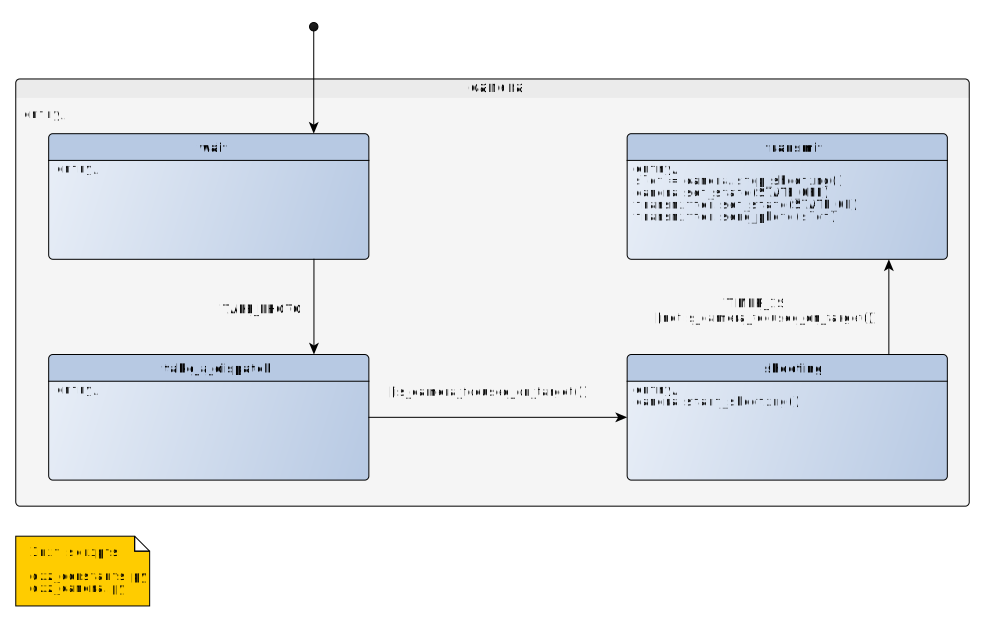
\includegraphics[width=15cm]{images/dzz-camera.eps}
    \caption{Диаграмма машины состояний для фотографирования объекта}
    \label{Pic:DZZ-camera}
  \end{flushright}
\end{figure}

Далее представлен код функции \verb'is_camera_focused_on_target', которая проверяет находится ли нужный нам объект на Земле в поле видимости камеры.

\begin{verbatim}
def is_camera_focused_on_target():
    a = navigation.get_z_axis_angle()
    return abs(a - target_angle) <= 1
\end{verbatim}

\section{SMS везде}

\paragraph{Условия миссии} В этой миссии КА стартует на орбите
заданной высоты. Необходимо будет получить сообщение с одной наземной станции и передать полученное сообщение другой наземной станции. КА должен будет обеспечить приём и передачу сообщений между \emph{18 станциями 5 раз}

\begin{figure}[tbh]
  \begin{center}
    \includegraphics[width=10cm]{images/sms.eps}
    \caption{КА в миссии «SMS везде»}
    \label{Pic:SMS}
  \end{center}
\end{figure}


\paragraph{Общая логика решения} 

\begin{enumerate}
\item Гашение начальной угловой скорости аппарата и выход на угловую скорость, необходимую для постоянного поддержания нормальной к земной поверхности ориентации;
\item когда КА соориентирован в надир, получаем сообщение от следующей по списку наземной станции;
\item когда сообщение получено целиком, прочитываем его и отсылаем станции-получателю;
\item повторяем 2 и 3 пункты еще 4 раза.
\end{enumerate}

Программа для установки КА в надир ничем не отличается от программы из первой тренировочной миссии. Нам остается лишь придумать как получать и отправлять сообщения в нужные наземные станции.

\paragraph{Высокопроизводительный канал связи} Следующая диаграмма (рисунок \ref{Pic:SMS-transmitter}) при получении события \verb'DELIVERY' начинает передавать сообщения станций друг другу. После получения события \verb'DELIVERY' каждый тик работы симулятора происходит проверка на полноту полученной информации от какой-то станции, и, если сообщение получено полностью, состояние подсистемы \verb'transmitter' переходит в \verb'get_message'. В данном состоянии подсистема читает полученное сообщение и переводит себя в состояние \verb'send_message', в котором отсылает сообщение нужной станции, при условии, что КА рядом с этой станцией. Данный цикл происходит до тех пор, пока не дойдет до последнего элемента в списке \verb'routing'.

\begin{figure}[tbh]
  \begin{center}
    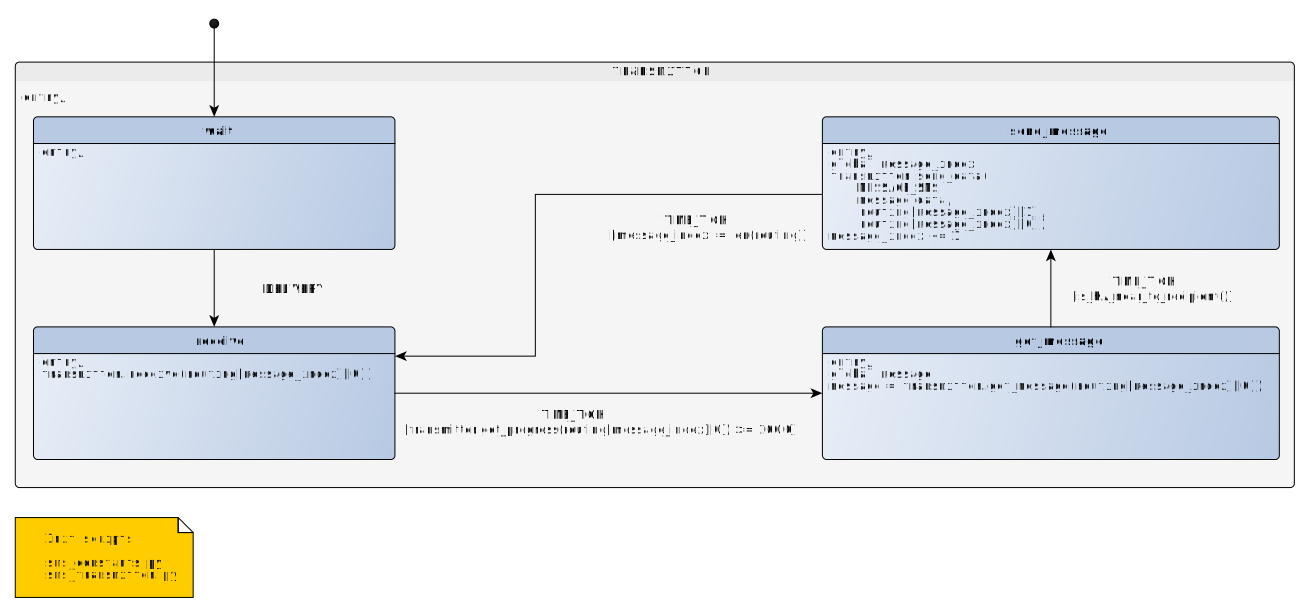
\includegraphics[width=15cm]{images/sms-transmitter.eps}
    \caption{Диаграмма машины состояний для передачи данных}
    \label{Pic:SMS-transmitter}
  \end{center}
\end{figure}


\section{Инспекция спутника}

\paragraph{Условия миссии} В этой миссии КА стартует на орбите
заданной высоты. Необходимо будет получить фотографию космического объекта в наилучшем качестве и передать полученное изображение в наземный измерительный пункт (\verb'НИП')

\begin{figure}[tbh]
  \begin{center}
    \includegraphics[width=12cm]{images/inspect.eps}
    \caption{КА в миссии «Инспекция спутника»}
    \label{Pic:Inspection}
  \end{center}
\end{figure}


\paragraph{Общая логика решения} 

Так как КА начинает миссию на различной от цели орбите, то качество снимка из-за расстояния будет низким. Поэтому для увеличения качества снимка нужно сократить это расстояние, т.е. перейти на орбиту цели.

\begin{enumerate}
\item Гашение начальной угловой скорости аппарата и выход на угловую скорость, необходимую для постоянного поддержания касательной к земной поверхности ориентации;
\item выход КА на орбиту космического объекта, когда космический объект находится на нужном для КА расстоянии для выполнения орбитального маневра, т.е. на таком расстоянии, при котором на новой орбите дистанция между нашим КА и целью была минимальна;
\item когда дистанция между КА и целью уменьшилась, соориентировать КА на цель и сфотографировать её;
\item передать полученную фотографию объекта в НИП через высокопроизводительный канал связи.
\end{enumerate}

\paragraph{Ориентация аппарата} Следующая диаграмма (рисунок \ref{Pic:INSPECT-orient}) стабилизирует, ориентирует касательно поверхности Земли, ориентирует на цель и ориентирует на любой желаемый угол.

\begin{figure}[tbh]
  \begin{center}
    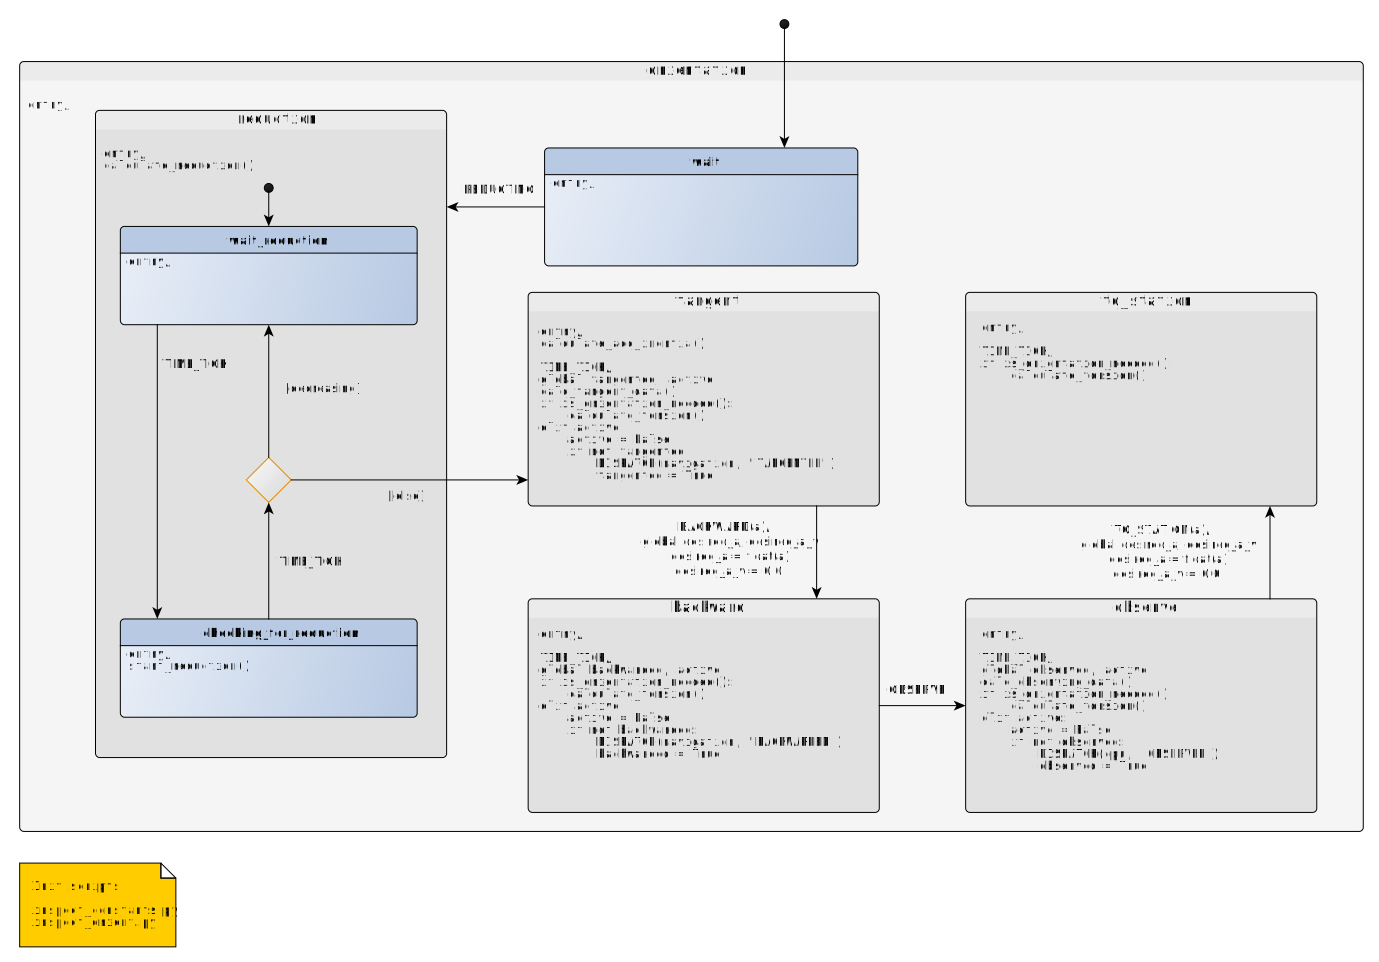
\includegraphics[width=15cm]{images/inspect-orient.eps}
    \caption{Диаграмма машины состояний для ориентации КА}
    \label{Pic:INSPECT-orient}
  \end{center}
\end{figure}

\begin{enumerate}
\item Стабилизация происходит в состоянии \verb'reduction' (модуль угловой скорости уменьшается до нуля).

\item В состоянии \verb'orienting' подсистема ориентации берет текущую угловую скорость и угол и превращает их в желаемую угловую скорость и в желаемый угол соответственно.

\item Ориентация касательно поверхности Земли происходит в состоянии \verb'tangent'. Желаемая угловая скорость и желаемый угол считаются так:
\begin{verbatim}
desired_a_v = -initial_nav_angular_velocity
desired_a = normalize_angle(360 - navigation.get_z_axis_angle())
\end{verbatim}
\item Ориентация на цель происходит в состоянии \verb'observing' благодаря функции \verb'calc_observing_data'.
\end{enumerate}

\clearpage

\paragraph{Условия. Проверка If/Else}Условия могут разделить исполнение программы на два потока с помощью служебного состояния условия, которое отображается с помощью примитива \textbf{BPMN Gateway} (рисунок \ref{Pic:IfElse})

\begin{figure}[tbh]
  \begin{center}
    \includegraphics[width=7.1cm]{images/diagrams-ifelse.eps}
    \caption{Проверка условий}
    \label{Pic:IfElse}
  \end{center}
\end{figure}

\paragraph{Навигация аппарата} Следующая диаграмма (рисунок \ref{Pic:INSPECT-navi}) управляет двигателем и расчитывает, когда он должен сделать двухимпульсный переход между орбитами.

\begin{figure}[tbh]
  \begin{center}
    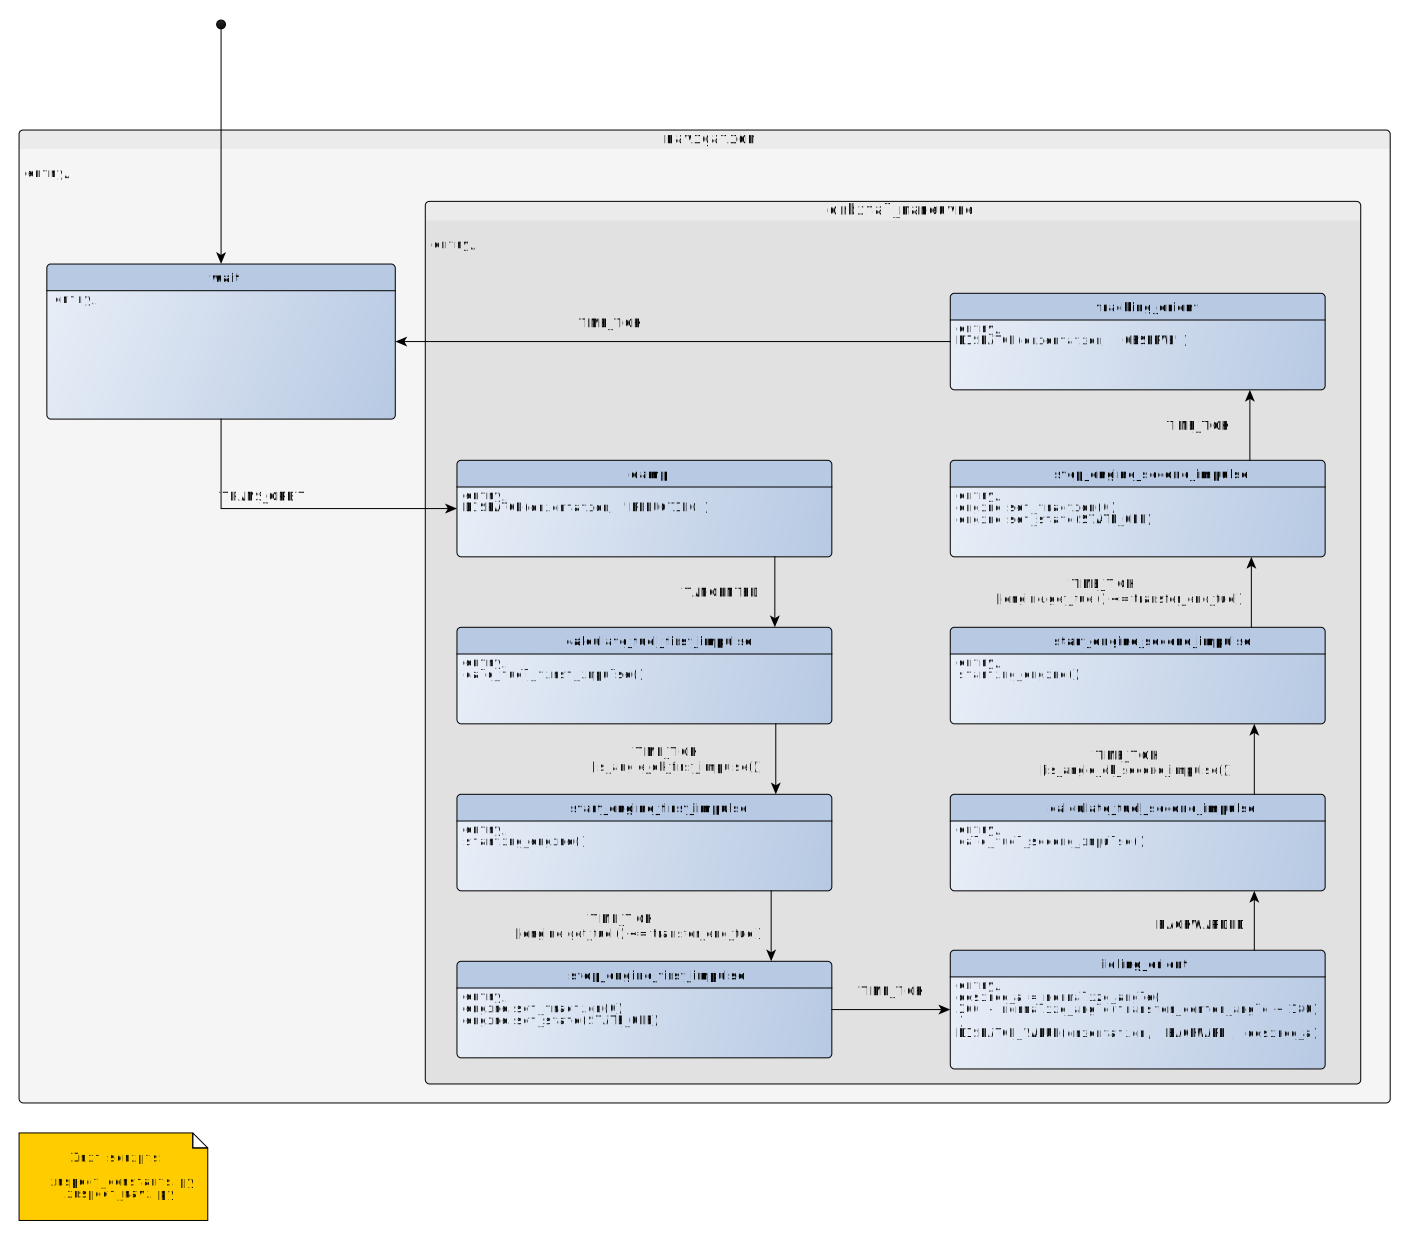
\includegraphics[width=15cm]{images/inspect-navi.eps}
    \caption{Диаграмма машины состояний для навигации КА}
    \label{Pic:INSPECT-navi}
  \end{center}
\end{figure}

Главным звеном в данной диаграмме является состояние \verb'impulse' подсистемы. В этом состоянии и происходит включение и выключение двигателя. Благодаря проверке \verb'is_angle_ok()' подсистема понимает когда нужно сделать импульс.

\section{Белковый кристалл в невеомости}

\paragraph{Условия миссии} В этой миссии КА стартует на орбите
заданной высоты. Необходимо с помощью специального оборудования в ограниченных условиях вырастить белковый кристалл, а затем отправить аппарат в заданную точку на поверхности Земли.

\begin{figure}[tbh]
  \begin{center}
    \includegraphics[width=12cm]{images/crystal.eps}
    \caption{КА в миссии «Белковый кристалл в невесомости»}
    \label{Pic:Crystal}
  \end{center}
\end{figure}

Успех миссии зависит от нескольких параметров. Во-первых, необходимо перевести КА на нужную орбиту $h_1$ с точностью 1 км для проведения эксперимента. Во-вторых для правильной работы научного оборудования необходимо будет отключить все подсистемы кроме полезной нагрузки и критически необходимых (БЦВМ, СЭП и СОТР). В-третьих, нужно будет поддерживать узкий диапазон критической температуры в течение одного оборота вокруг Земли, что особенно важно для полезной нагрузки. Совершив один оборот по заданной орбите, аппарат может включать назад все системы и отправляться на Землю, где он должен совершить посадку как можно ближе к требуемой точке.

\clearpage
\paragraph{Общая логика решения} 

\begin{enumerate}
\item Гашение начальной угловой скорости аппарата и выход на угловую скорость, необходимую для постоянного поддержания касательной к земной поверхности ориентации;
\item выход КА на орбиту космического объекта, когда космический объект находится на нужном для КА расстоянии для выполнения орбитального маневра, т.е. на таком расстоянии, при котором на новой орбите дистанция между нашим КА и целью была минимальна;
\item когда дистанция между КА и целью уменьшилась, соориентировать КА на цель и сфотографировать её;
\item передать полученную фотографию объекта в НИП через высокопроизводительный канал связи.
\end{enumerate}

\paragraph{Падение исследовательского контейнера} Следующая диаграмма (рисунок \ref{Pic:Сrystal-navi-conteinre-fall}) сбрасывает исследовательский контейнер на нужное место на Земле.

\begin{figure}[tbh]
  \begin{center}
    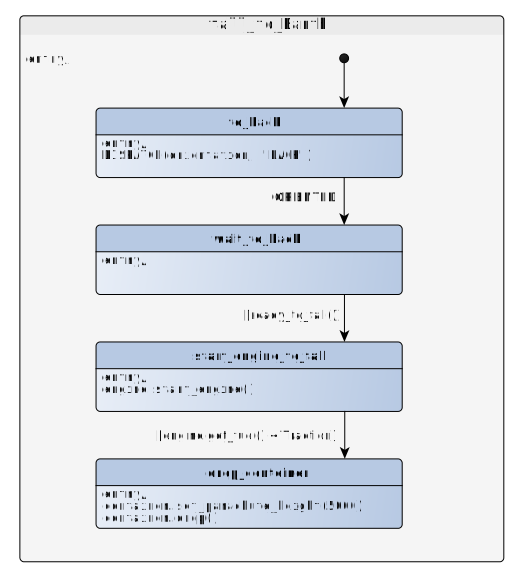
\includegraphics[width=10cm]{images/crystal-navi-conteiner-fall.eps}
    \caption{Диаграмма машины состояний для падения контейнера с орбиты}
    \label{Pic:Сrystal-navi-conteinre-fall}
  \end{center}
\end{figure}

КА снижает скорость и сбрасывает контейнер

\section{Спутник связи <<Молния>>}

\paragraph{Условия миссии} В этой миссии КА стартует на орбите
заданной высоты. Необходимо, имея ограниченный ресурс по топливу и параметрам спутника, организовать несколько сеансов продолжительной радиосвязи с наземным измерительным пунктом.

\begin{figure}[tbh]
  \begin{center}
    \includegraphics[width=10cm]{images/molniya.eps}
    \caption{Соотношение круговой орбиты и орбиты «Молния»}
    \label{Pic:Molniya}
  \end{center}
\end{figure}

Космический аппарат находится на круговой низкой орбите. Чтобы провести сеанс связи длительностью не менее 8 часов, в ходе миссии нужно будет перевести спутник на подходящую эллиптическую
орбиту.

\clearpage
\paragraph{Общая логика решения} 

\begin{enumerate}
\item Гашение начальной угловой скорости аппарата и выход на угловую скорость, необходимую для постоянного поддержания касательной к земной поверхности ориентации;
\item переход на эллиптическую орбиту;
\item поддержка сеанса связи космического аппарата с НИП
\end{enumerate}

\paragraph{Навигация КА} Следующая диаграмма (рисунок \ref{Pic:Molniya-navi}) переводит наш космический аппарат с низкой орбиты на эллиптическую.

\begin{figure}[tbh]
  \begin{center}
    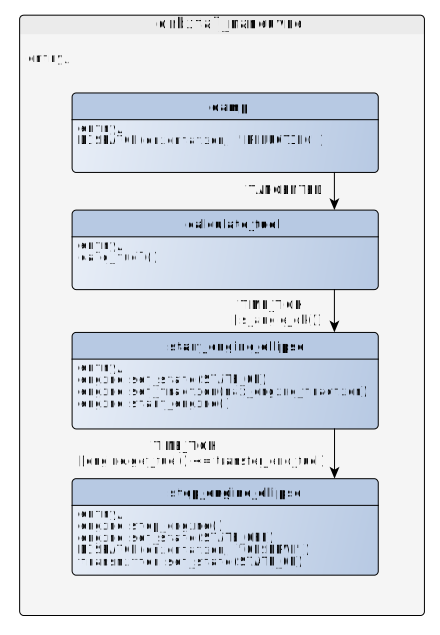
\includegraphics[width=8.5cm]{images/molniya-navi.eps}
    \caption{Диаграмма машины состояний для навигации КА}
    \label{Pic:Molniya-navi}
  \end{center}
\end{figure}

Здесь, после получения события \verb'TANGENTED' от подсистемы ориентации, начинается переход на эллиптическую орбиту. Как только двигатель космического аппарата истратит нужный объем топлива, посчитанный в функции \verb'calc_fuel()', двигатель выключится, и подсистема навигации отправит событие \verb'SET_STAGE' в подсистему ориентации для поддержки ориентации на Землю

\clearpage
\paragraph{Поддержка ориентации на Землю} Следующая диаграмма (рисунок \ref{Pic:Molniya-navi}) поддерживает ориентацию на Землю

\begin{figure}[tbh]
  \begin{center}
    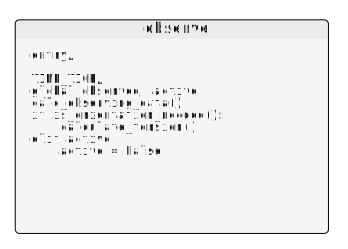
\includegraphics[width=14cm]{images/molniya-orient.eps}
    \caption{Диаграмма машины состояний для ориентации КА на Землю}
    \label{Pic:Molniya-navi}
  \end{center}
\end{figure}

Здесь происходит высчитывание нужного угла и угловой скорости и корректировка ориентации по полученым значениям.
Ориентация на Землю начинается только в тот момент времени, когда было получено событие \verb'SET_STAGE' со значением 3 или тогда, когда значение глобальной переменной \verb'stage' равно 3.
   
\section*{Перечень сокращений}
\addcontentsline{toc}{section}{Перечень сокращений}

\begin{description}
\item[БЦВМ] бортовая центральная вычислительная машина;
\item[ДЗЗ] дистанционное зондирование Земли;
\item[ИСЗ] искусственный спутник Земли;
\item[КА] космический аппарат;
\item[НИП] наземный измерительный пункт;
\item[СКО] система коррекции орбиты;
\item[СН] систем навигации;
\item[СОТР] система обеспечения теплового режима;
\item[СТМИ] система телеметрии;
\item[СУОС] система управления ориентацией и стабилизацией;
\item[СЭП] система электропитания;
\item[ФЭП] фотоэлектрические элементы.
\end{description}

\begin{thebibliography}{2}
\addcontentsline{toc}{section}{Список литературы и материалов}
\bibitem{CRASHCOURSE} Samek M., A Crash Course in UML State Machines~---
  \url{https://www.state-machine.com/doc/AN_Crash_Course_in_UML_State_Machines.pdf}
\end{thebibliography}

\clearpage
\section*{Приложение 1: Инструкция по инструментам программирования}
\addcontentsline{toc}{section}{Приложение 1: Инструкция по инструментам программирования}

\subsection*{Создание диаграмм}
\addcontentsline{toc}{subsection}{Создание диаграмм}

Для работы с диаграммами состояний в симуляторе ОРБИТА 2.0 вам необходимо создать
диаграмму в редакторе \textbf{yEd} с применением следующих ограничений.

Диаграммы должны содержать следующие базовые примитивы:

\begin{description}
\item[Атомарное состояние] Самый простой блок диаграммы~--- состояние, которое не содержит
  в себе других состояний. Изображается посредством примитива \textbf{Entity Relationship}
  с обозначением названия состояния в заголовке и триггеров в теле блока.

\begin{figure}[h]
  \begin{center}
    \includegraphics[width=6cm]{images/diagrams-state.eps}
  \end{center}
\end{figure}

\item[Родительское состояние] Иерархический блок диаграммы, который содержит в себе другие
  состояния. Изображается посредством примитива \textbf{Group Node}. Аналогичным образом
  содержит название состояния в заголовке и описание триггеров в теле блока.

\begin{figure}[h]
  \begin{center}
    \includegraphics[width=6cm]{images/diagrams-hstate.eps}
  \end{center}
\end{figure}

\item[Начальное состояние] Стартовое состояние как для всей диаграммы, так и для
  определения старта для дочерних состояний внутри родительского. Изображается посредством
  примитива \textbf{BPMN Plain Event} и в соответствии со стандартом UML 2.0 выглядит как
  черный кружок.
  
\begin{figure}[h]
  \begin{center}
    \includegraphics[width=0.3cm]{images/diagrams-start.eps}
  \end{center}
\end{figure}
  
\item[События / переходы] Представляют собой события с соответствующими параметрами,
  описанными выше. Изображаются посредством стандартных переходов \textbf{Edge}.

\begin{figure}[h]
  \begin{center}
    \includegraphics[width=6cm]{images/diagrams-transition.eps}
  \end{center}
\end{figure}
  
\item[Заключительные состояния] Заключительное состояние для диаграммы, может не
  включаться в диаграмму полета КА. Изображается посредством примитива \textbf{BPMN
    Terminate Event}.

\begin{figure}[h]
  \begin{center}
    \includegraphics[width=2cm]{images/diagrams-finish.eps}
  \end{center}
\end{figure}

\item[Условия] Условия могут разделить исполнение программы на два потока с помощью
  служебного состояния условия, которое отображается с помощью примитива \textbf{BPMN
    Gateway}.
  
\begin{figure}[h]
  \begin{center}
    \begin{subfigure}{0.4\textwidth}
      \includegraphics[width=5cm]{images/diagrams-ifelse.eps}
    \end{subfigure}
    \hfill
    \begin{subfigure}{0.4\textwidth}
      \includegraphics[width=4cm]{images/diagrams-note.eps}
    \end{subfigure}
  \end{center}
\end{figure}

\item[Технические описания] Дополнительное поля, необходимые для создания корректной
  программы полета. Могут содержать справочную информацию для разработчиков и специальную
  информацию для генератора кода. В текущей версии существует два варианта необязательных
  служебных полей с заголовками: \verb'Initialization:', содержащим код инициализации для
  программы на Python, и \verb'Init scripts:', содержащим список импортируемых модулей на
  языке Python. Изображаются посредством примитива \textbf{UML Note}.

\end{description}

Мы рекомендуем использовать существующие примеры (например, см. директории
\verb'models/earth/probes/' и \verb'models/earth/sm/test/graphs/') для создания диаграмм
полета на их основе.

\subsection*{Включение диаграмм в описание аппарата}
\addcontentsline{toc}{subsection}{Включение диаграмм в описание аппарата}

Описания конструкции и программ КА, условий всего полёта содержатся в XML-файле,
соответствующем описанию в \verb'/models/earth/xml-schemas/probes.xsd'. Примеры готовых
аппаратов можно найти в директории \verb'/models/earth/probes'.

В описании аппарата есть раздел, посвященный отдельным подсистемам. Вместо указания кода
на языке Python можно следующим образом привязывать диаграммы состояний к подсистемам КА:

\begin{verbatim}
<systems>
  <system name="Cubesat-Case-3U"/>
  <system name="Orient-2" start_mode="ON">
    <hsm_diagram type="yEd" path="test2sm-orient.graphml"/>
  </system>
  <system name="Telemetry-1" start_mode="ON"/>
  <system name="Navi-1" start_mode="ON"/>
  <system name="Power-1" start_mode="ON"/>
  <system name="Therm-1" start_mode="ON">
    <hsm_diagram type="yEd" path="test2sm-heat.graphml"/>
  </system>
  <system name="Radio-1" start_mode="OFF"/>
  <system name="CPU-1" start_mode="ON">
    <hsm_diagram type="yEd" path="test2sm-main.graphml"/>
  </system>
</systems>
\end{verbatim}

Файлы с диаграммами в формате \verb'.graphml' должны находиться в той же директории, что и
описание аппарата, или в атрибуте \verb'path' нужно указать полный путь до диаграммы.

\subsection*{Инструменты для тестирования диаграмм}
\addcontentsline{toc}{subsection}{Инструменты для тестирования диаграмм}

В директории \verb'/models/earth/sm/test' расположены скрипты для тестирования машин
состояний. Там же можно найти примеры тестовых диаграмм, реализующих базовую
функциональность машин состояний.

Для освоения языка диаграмм машин состояний рекомендуется использовать
специальный скрипт \verb'run.py', с помощью которого можно <<запустить>> любую диаграмму
без симулятора КА. При этом нужно учитывать ряд ограничений:

\begin{itemize}
\item верхнеуровневое состояние в диаграмме должно называться \verb'cpu';
\item в диаграмме должно быть стартовое состояние;
\item вам придется использовать функцию \verb'debug(str)' для вывода сообщений в консоль;
\item вы можете использовать событие \verb'GETCHAR' с параметром для получения символа с
  клавиатуры (см. пример диаграммы \verb'/sm/test/graph/getchar.graphml').
\end{itemize}

Например, при запуске диаграммы, представленной на рисунке \ref{Pic:TestDiagr}) будет получен следующий результат:

\begin{figure}[tbh]
  \begin{center}
    \includegraphics[width=15cm]{images/test-diagram.eps}
    \caption{Пример пробной диаграммы}
    \label{Pic:TestDiagr}
  \end{center}
\end{figure}

\begin{verbatim}
INIT
ENTRY A
ENTRY B
ENTRY C
TERM
\end{verbatim}

Если же вы захотите протестировать полноценную программу полета с обращением к функциям
подсистем КА, рекомендуем воспользоваться тестовым API (\verb'/models/earth/api-test') и
реализовать в нем все необходимые функции.

\end{document}
